\documentclass{beamer}
\usepackage{graphicx}

\setbeamertemplate{section in toc}[sections numbered]
\setbeamertemplate{subsection in toc}[subsections numbered]
\setbeamertemplate{page number in toc}[totalframenumber]

\setbeamertemplate{footline}{
  \hspace*{0.2cm} 
  \insertframenumber/\inserttotalframenumber 
}

\title{1. domača naloga pri predmetu napredna računalniška orodja}
\author{Aljaž Luznar}
\institute{Univerza v ljubljani Fakulteta za strojništvo}
\date{\today}

\begin{document}

\frame{\titlepage}

\begin{frame}{Kazalo}
    \tableofcontents
\end{frame}

\logo{
\includegraphics[width=1.5cm]{logo.jpg}}

\section{Predstavitev Monte Carlo metode za izračun vrednosti $\pi$}
\begin{frame}{Predstavitev Monte Carlo metode za izračun vrednosti $\pi$}
    \begin{itemize}
        \item Ustvaril sem funkcijsko datoteko mcc\_pi.m, ki ima kot vhodni parameter število točk, vrne pa nam pa koordinate točk znotraj kroga in koordinate točk znotraj kvadrata.
    \begin{figure}
        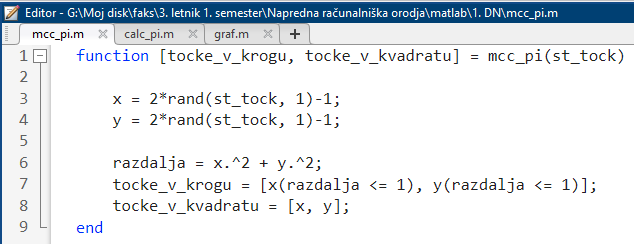
\includegraphics[width=0.7\textwidth]{Posnetek zaslona 2023-10-22 162922.png}
        \caption{koda za funkcijo mcc\_pi.m}
    \end{figure}

    \end{itemize}
\end{frame}
\begin{frame}{Predstavitev Monte Carlo metode za izračun vrednosti $\pi$}
    \begin{itemize}
        \item Nato sem ustvaril programsko datoteko calc\_pi.m. Datoteka vsebuje funkcijo area\_pi.m. Funkcija izračuna število $\pi$ na podlagi Monte Carlo metode in vrne napako izračuna.
    \begin{figure}
        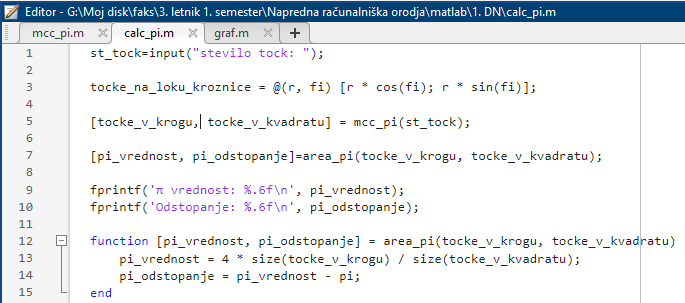
\includegraphics[width=0.7\textwidth]{Posnetek zaslona 2023-10-22 163758.png}
        \caption{koda za funkcijo calc\_pi.m}
    \end{figure}

    \end{itemize}
\end{frame}

\section{Rezultati izračuna}
\begin{frame}{Rezultati izračuna}
    \begin{itemize}
        \item Rezultate prikažemo s pomočjo programa na spodnjo sliki.
    \begin{figure}
        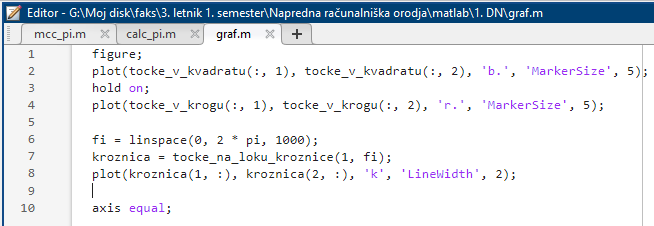
\includegraphics[width=0.7\textwidth]{Posnetek zaslona 2023-10-22 171843.png}
        \caption{koda za prikaz rezultativ}
    \end{figure}
    \end{itemize}
\end{frame}
\begin{frame}{Rezultati izračuna}
    \begin{itemize}
        \item Pri vrednosti 1000 točk dobimo naslednji graf (verzija kode grafa z označenimi osmi je naložena v mojem GitHubu)
    \begin{figure}
        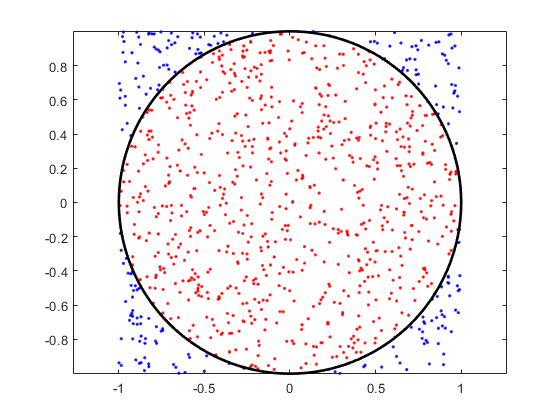
\includegraphics[width=0.7\textwidth]{123.png}
        \caption{koda za prikaz rezultativ}
    \end{figure}
    \end{itemize}
\end{frame}
\begin{frame}{Rezultati izračuna}
    \begin{itemize}
        \item S spreminjanjem števila točk dobimo naslenje rezultate in odstopke. Ugotovimo da se z povečenanjem števila točk veča natančnost izračuna. 
        \pause
        \item 10 točk: 3.615385 napaka: 0.473792 \\100 točk: 2.880448 napaka: -0.261145 \\1000 točk: 3.080004 napaka: -0.061589\\ 10000 točk: 3.162000 napaka: 0.020407
    \end{itemize}
\end{frame}

\section{Git}
\begin{frame}{Git}
    \begin{itemize}
        \item Vse datoteke uporabljene v tej nalogi sem naložil na svoj Git profil.
    \end{itemize}
\end{frame}


\section{Beamer}
\begin{frame}{Beamer}
    \begin{itemize}
        \item Za del naloge ki zahteva uporabo orodja Beamer sem izdelal to predstavitev.
    \end{itemize}
\end{frame}

\end{document}